\clearpage
\section*{2025.4.12 高数辅导}
\setstretch{1.75}

\begin{example}
    {1}{
        求$I= \int_{L} (x+y)^3 ~\d x - (x-y)^3 ~\d y$，
        其中$L$为图$4$所示的两个上半圆周连成的曲线$AOB$.
    }
\end{example}

\begin{figure}[H] 
    \centering
    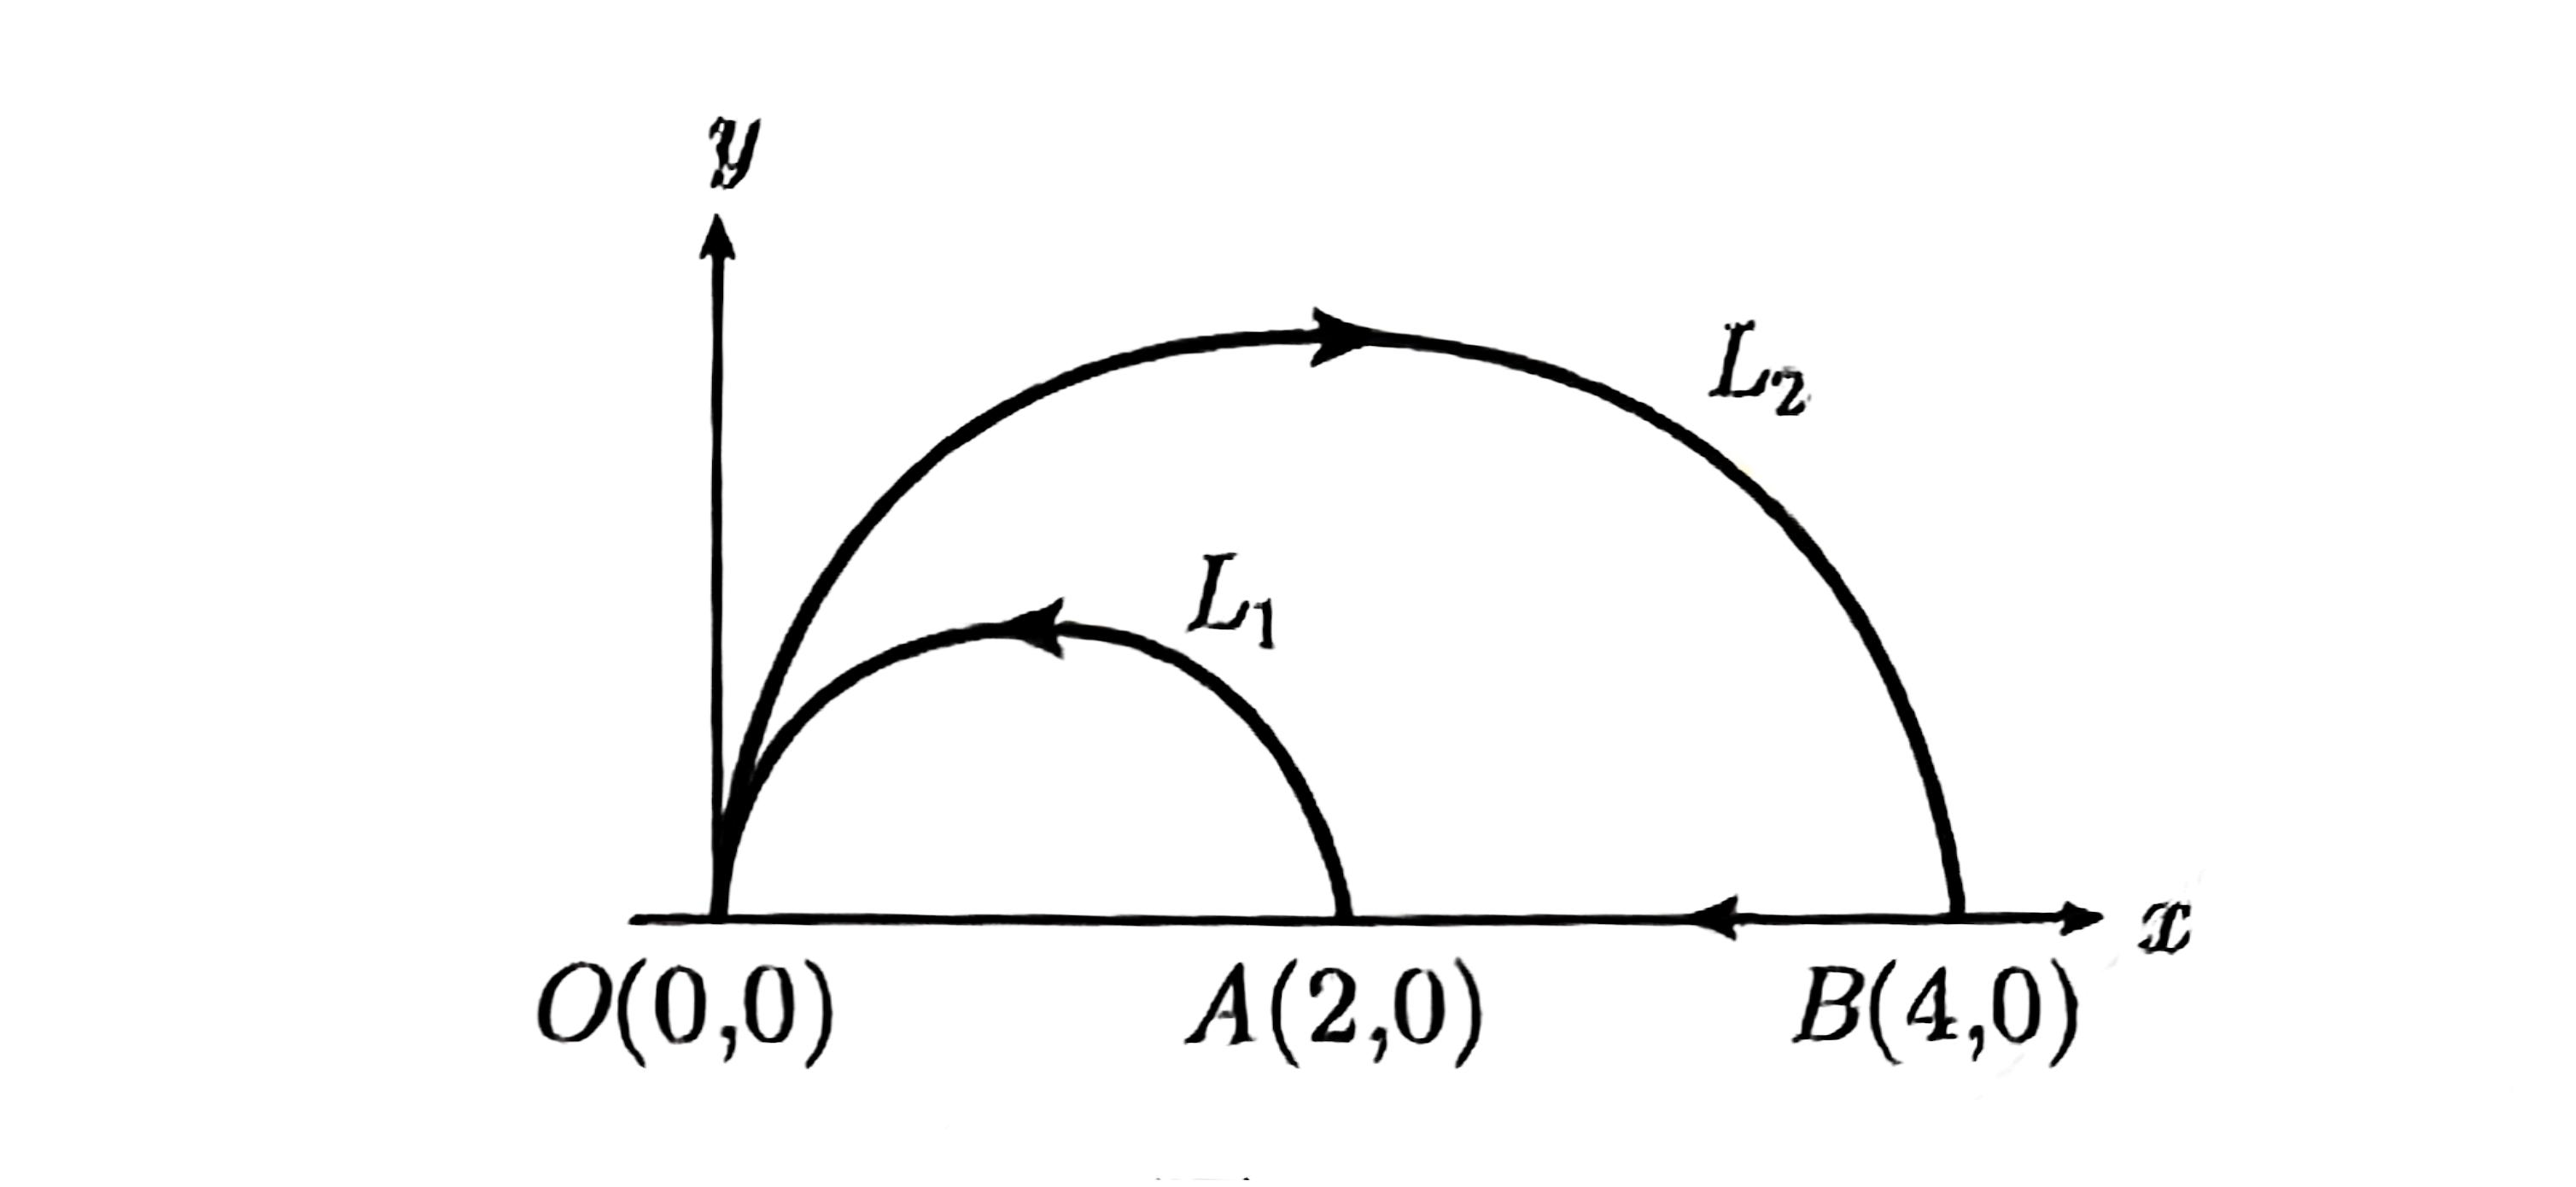
\includegraphics[width=0.5\textwidth]{fig8-4.jpg}
    \caption{例1题图} 
\end{figure}\par

\clearpage


\begin{example}
    {2}{
        计算积分$I = \oint_\varGamma \left( \frac{y^2 + y + 4x^2}{4x^2 + y^2} + \sin x^2 \right)~\d x + \left( \frac{4x^2 - x + y^2}{4x^2 + y^2} + \sin y^2 \right)~\d y,$
其中闭曲线 \(\varGamma\) 由上半圆 \(x^2 + y^2 = 9 \ (y \ge 0)\) 和下半椭圆 \(\frac{x^2}{9} + \frac{y^2}{16} = 1 \ (y \le 0)\) 组成，方向为逆时针.
    }
\end{example}\par
~\par

\clearpage

\textbf{例3}~~\textit{设曲面 \( S \) 是柱体  
    $\Omega = \{(x,y,z) \mid x^2 + y^2 \leq 1, \, 0 \leq z \leq 1\}$
    表面的外侧（同时包含上表面、下表面、侧面）.}
    \textit{计算下列积分：}
    
    \textit{(a)} $I_1 = \iint_S (y - z) |x| \, \d y \, \d z + (z - x)|y| \, \d z \, \d x + (x - y)|z| \, \d x \, \d y$;\vspace{0.25em}
    
    \textit{(b)} $I_2 = \iint_S (y - z)x^2 \, \d y \, \d z + (z - x)y^2 \, \d z \, \d x + (x - y)z^2 \, \d x \, \d y$;\vspace{0.25em}
    
    \textit{(c)} $I_3 = \iint_S (y - z)x^3 \, \d y \, \d z + (z - x)y^3 \, \d z \, \d x + (x - y)z^3 \, \d x \, \d y$.\vspace{0.25em}\par
~\par

\clearpage

\textbf{例4}~~\textit{设$f(x)$为$\mathbb{R}$上的一元函数，证明：}
\begin{eq}
    \iint_{S} f(x+y+z)~\d S = 2\pi \int_{-1}^{1} f(\sqrt{3} \xi) ~\d \xi
\end{eq}
其中$S$为单位球面$x^2 + y^2 + z^2 = 1$.\par
~\par

\clearpage

\textbf{例5}~~

\textit{(1)~设$D =   \mathbb{R}^2 -\left\{  (x,0) \mid x \ge 0 \right\}$. 写出一个函数$T:D \to \mathbb{R}$
满足$T$在$D$中处处可微，并且：}
\begin{eq}
    \frac{\partial T}{\partial x} = -\frac{y}{x^2 + y^2},~~\frac{\partial T}{\partial y} = \frac{x}{x^2 + y^2}
\end{eq}

\textit{(2)~设$\Omega = \mathbb{R}^2 - \left\{ 0 \right\}$.
证明不存在函数$U:\Omega \to \mathbb{R}$，满足$U$在$\Omega$中每点可微，并且：}
\begin{eq}
    \frac{\partial U}{\partial x} = -\frac{y}{x^2 + y^2},~~\frac{\partial U}{\partial y} = \frac{x}{x^2 + y^2}
\end{eq}